\documentclass{standalone}
\usepackage{tikz}
\usetikzlibrary{patterns, positioning}


\begin{document}
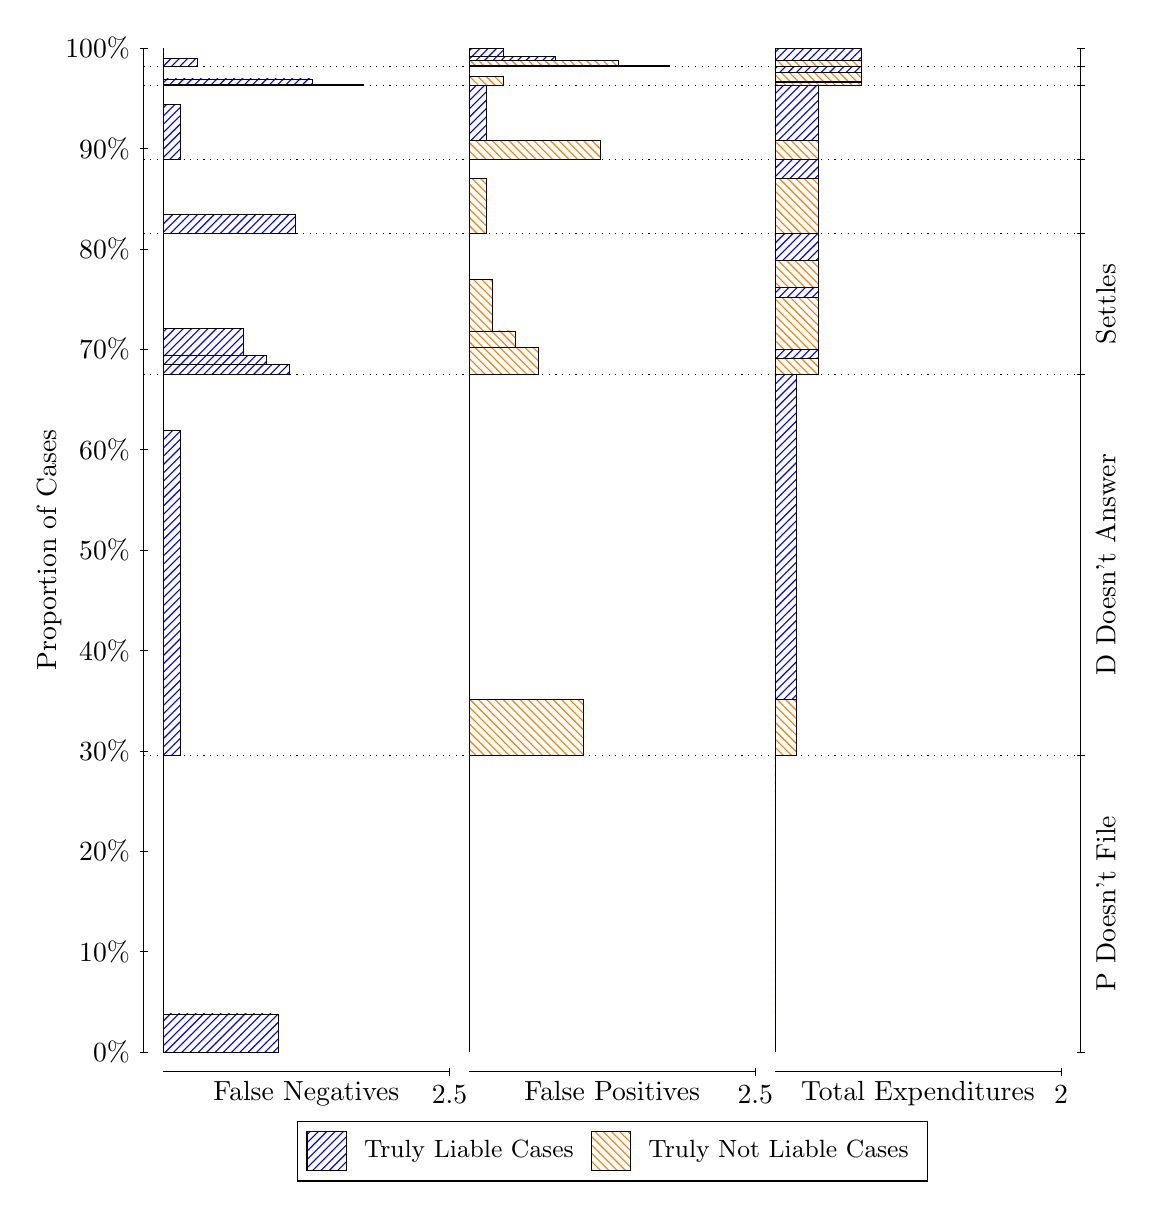
\begin{tikzpicture}
\draw[black, very thin] (1.5,1.75) -- (1.5,14.5);
\node[rotate=90, text=black, anchor=center] at (0.3, 8.125) {Proportion of Cases};
\draw[black, very thin] (1.45,1.75) -- (1.55,1.75);
\node[text=black, anchor=east] at (1.45, 1.75) {0\%};
\draw[black, very thin] (1.45,3.025) -- (1.55,3.025);
\node[text=black, anchor=east] at (1.45, 3.025) {10\%};
\draw[black, very thin] (1.45,4.3) -- (1.55,4.3);
\node[text=black, anchor=east] at (1.45, 4.3) {20\%};
\draw[black, very thin] (1.45,5.575) -- (1.55,5.575);
\node[text=black, anchor=east] at (1.45, 5.575) {30\%};
\draw[black, very thin] (1.45,6.85) -- (1.55,6.85);
\node[text=black, anchor=east] at (1.45, 6.85) {40\%};
\draw[black, very thin] (1.45,8.125) -- (1.55,8.125);
\node[text=black, anchor=east] at (1.45, 8.125) {50\%};
\draw[black, very thin] (1.45,9.4) -- (1.55,9.4);
\node[text=black, anchor=east] at (1.45, 9.4) {60\%};
\draw[black, very thin] (1.45,10.675) -- (1.55,10.675);
\node[text=black, anchor=east] at (1.45, 10.675) {70\%};
\draw[black, very thin] (1.45,11.95) -- (1.55,11.95);
\node[text=black, anchor=east] at (1.45, 11.95) {80\%};
\draw[black, very thin] (1.45,13.225) -- (1.55,13.225);
\node[text=black, anchor=east] at (1.45, 13.225) {90\%};
\draw[black, very thin] (1.45,14.5) -- (1.55,14.5);
\node[text=black, anchor=east] at (1.45, 14.5) {100\%};

\draw[black, very thin] (13.4,1.75) -- (13.4,14.5);
\draw[black, very thin] (13.35,1.75) -- (13.45,1.75);
\node[anchor=west] at (13.35, 1.75) {};
\draw[black, very thin] (13.35,5.5119) -- (13.45,5.5119);
\node[anchor=west] at (13.35, 5.5119) {};
\draw[black, very thin] (13.35,10.359) -- (13.45,10.359);
\node[anchor=west] at (13.35, 10.359) {};
\draw[black, very thin] (13.35,12.142) -- (13.45,12.142);
\node[anchor=west] at (13.35, 12.142) {};
\draw[black, very thin] (13.35,13.083) -- (13.45,13.083);
\node[anchor=west] at (13.35, 13.083) {};
\draw[black, very thin] (13.35,14.025) -- (13.45,14.025);
\node[anchor=west] at (13.35, 14.025) {};
\draw[black, very thin] (13.35,14.262) -- (13.45,14.262);
\node[anchor=west] at (13.35, 14.262) {};
\draw[black, very thin] (13.35,14.5) -- (13.45,14.5);
\node[anchor=west] at (13.35, 14.5) {};

\draw[black, very thin, pattern color=blue, pattern=north east lines] (1.75,1.75) rectangle (3.2033,2.2345);
\draw[black, very thin, pattern color=orange, pattern=north west lines] (1.75,2.2345) rectangle (1.75,5.5119);
\draw[black, very thin, pattern color=blue, pattern=north east lines] (1.75,5.5119) rectangle (1.968,9.6455);
\draw[black, very thin, pattern color=orange, pattern=north west lines] (1.75,9.6455) rectangle (1.75,10.359);
\draw[black, very thin, pattern color=blue, pattern=north east lines] (1.75,10.359) rectangle (3.3487,10.482);
\draw[black, very thin, pattern color=blue, pattern=north east lines] (1.75,10.482) rectangle (3.058,10.593);
\draw[black, very thin, pattern color=blue, pattern=north east lines] (1.75,10.593) rectangle (2.7673,10.936);
\draw[black, very thin, pattern color=orange, pattern=north west lines] (1.75,10.936) rectangle (1.75,12.142);
\draw[black, very thin, pattern color=blue, pattern=north east lines] (1.75,12.142) rectangle (3.4213,12.384);
\draw[black, very thin, pattern color=orange, pattern=north west lines] (1.75,12.384) rectangle (1.75,13.083);
\draw[black, very thin, pattern color=blue, pattern=north east lines] (1.75,13.083) rectangle (1.968,13.782);
\draw[black, very thin, pattern color=orange, pattern=north west lines] (1.75,13.782) rectangle (1.75,14.025);
\draw[black, very thin, pattern color=blue, pattern=north east lines] (1.75,14.025) rectangle (4.2933,14.037);
\draw[black, very thin, pattern color=blue, pattern=north east lines] (1.75,14.037) rectangle (3.6393,14.108);
\draw[black, very thin, pattern color=orange, pattern=north west lines] (1.75,14.108) rectangle (1.75,14.262);
\draw[black, very thin, pattern color=blue, pattern=north east lines] (1.75,14.262) rectangle (2.186,14.373);
\draw[black, very thin, pattern color=orange, pattern=north west lines] (1.75,14.373) rectangle (1.75,14.457);
\draw[black, very thin, pattern color=blue, pattern=north east lines] (1.75,14.457) rectangle (1.75,14.5);
\draw[black, very thin, pattern color=orange, pattern=north west lines] (5.6333,1.75) rectangle (5.6333,5.0274);
\draw[black, very thin, pattern color=blue, pattern=north east lines] (5.6333,5.0274) rectangle (5.6333,5.5119);
\draw[black, very thin, pattern color=orange, pattern=north west lines] (5.6333,5.5119) rectangle (7.0867,6.2249);
\draw[black, very thin, pattern color=blue, pattern=north east lines] (5.6333,6.2249) rectangle (5.6333,10.359);
\draw[black, very thin, pattern color=orange, pattern=north west lines] (5.6333,10.359) rectangle (6.5053,10.702);
\draw[black, very thin, pattern color=orange, pattern=north west lines] (5.6333,10.702) rectangle (6.2147,10.908);
\draw[black, very thin, pattern color=orange, pattern=north west lines] (5.6333,10.908) rectangle (5.924,11.564);
\draw[black, very thin, pattern color=blue, pattern=north east lines] (5.6333,11.564) rectangle (5.6333,12.142);
\draw[black, very thin, pattern color=orange, pattern=north west lines] (5.6333,12.142) rectangle (5.8513,12.841);
\draw[black, very thin, pattern color=blue, pattern=north east lines] (5.6333,12.841) rectangle (5.6333,13.083);
\draw[black, very thin, pattern color=orange, pattern=north west lines] (5.6333,13.083) rectangle (7.3047,13.326);
\draw[black, very thin, pattern color=blue, pattern=north east lines] (5.6333,13.326) rectangle (5.8513,14.025);
\draw[black, very thin, pattern color=orange, pattern=north west lines] (5.6333,14.025) rectangle (6.0693,14.136);
\draw[black, very thin, pattern color=orange, pattern=north west lines] (5.6333,14.136) rectangle (5.6333,14.179);
\draw[black, very thin, pattern color=blue, pattern=north east lines] (5.6333,14.179) rectangle (5.6333,14.262);
\draw[black, very thin, pattern color=orange, pattern=north west lines] (5.6333,14.262) rectangle (8.1767,14.275);
\draw[black, very thin, pattern color=orange, pattern=north west lines] (5.6333,14.275) rectangle (7.5227,14.346);
\draw[black, very thin, pattern color=blue, pattern=north east lines] (5.6333,14.346) rectangle (6.7233,14.389);
\draw[black, very thin, pattern color=blue, pattern=north east lines] (5.6333,14.389) rectangle (6.0693,14.5);
\draw[black, very thin, pattern color=orange, pattern=north west lines] (9.5167,1.75) rectangle (9.5167,5.0274);
\draw[black, very thin, pattern color=blue, pattern=north east lines] (9.5167,5.0274) rectangle (9.5167,5.5119);
\draw[black, very thin, pattern color=orange, pattern=north west lines] (9.5167,5.5119) rectangle (9.7892,6.2249);
\draw[black, very thin, pattern color=blue, pattern=north east lines] (9.5167,6.2249) rectangle (9.7892,10.359);
\draw[black, very thin, pattern color=orange, pattern=north west lines] (9.5167,10.359) rectangle (10.062,10.565);
\draw[black, very thin, pattern color=blue, pattern=north east lines] (9.5167,10.565) rectangle (10.062,10.676);
\draw[black, very thin, pattern color=orange, pattern=north west lines] (9.5167,10.676) rectangle (10.062,11.332);
\draw[black, very thin, pattern color=blue, pattern=north east lines] (9.5167,11.332) rectangle (10.062,11.456);
\draw[black, very thin, pattern color=orange, pattern=north west lines] (9.5167,11.456) rectangle (10.062,11.799);
\draw[black, very thin, pattern color=blue, pattern=north east lines] (9.5167,11.799) rectangle (10.062,12.142);
\draw[black, very thin, pattern color=orange, pattern=north west lines] (9.5167,12.142) rectangle (10.062,12.841);
\draw[black, very thin, pattern color=blue, pattern=north east lines] (9.5167,12.841) rectangle (10.062,13.083);
\draw[black, very thin, pattern color=orange, pattern=north west lines] (9.5167,13.083) rectangle (10.062,13.326);
\draw[black, very thin, pattern color=blue, pattern=north east lines] (9.5167,13.326) rectangle (10.062,14.025);
\draw[black, very thin, pattern color=orange, pattern=north west lines] (9.5167,14.025) rectangle (10.607,14.068);
\draw[black, very thin, pattern color=blue, pattern=north east lines] (9.5167,14.068) rectangle (10.607,14.08);
\draw[black, very thin, pattern color=orange, pattern=north west lines] (9.5167,14.08) rectangle (10.607,14.191);
\draw[black, very thin, pattern color=blue, pattern=north east lines] (9.5167,14.191) rectangle (10.607,14.262);
\draw[black, very thin, pattern color=orange, pattern=north west lines] (9.5167,14.262) rectangle (10.607,14.346);
\draw[black, very thin, pattern color=blue, pattern=north east lines] (9.5167,14.346) rectangle (10.607,14.5);
\draw[black, dotted] (1.5,5.5119) -- (13.4,5.5119);
\draw[black, dotted] (1.5,10.359) -- (13.4,10.359);
\draw[black, dotted] (1.5,12.142) -- (13.4,12.142);
\draw[black, dotted] (1.5,13.083) -- (13.4,13.083);
\draw[black, dotted] (1.5,14.025) -- (13.4,14.025);
\draw[black, dotted] (1.5,14.262) -- (13.4,14.262);
\draw[black, very thin] (1.75,1.5) -- (5.3833,1.5);
\node[text=black, anchor=north] at (3.5667, 1.5) {False Negatives};
\draw[black, very thin] (5.3833,1.45) -- (5.3833,1.55);
\node[text=black, anchor=north] at (5.3833, 1.45) {2.5};

\draw[black, very thin] (5.6333,1.5) -- (9.2667,1.5);
\node[text=black, anchor=north] at (7.45, 1.5) {False Positives};
\draw[black, very thin] (9.2667,1.45) -- (9.2667,1.55);
\node[text=black, anchor=north] at (9.2667, 1.45) {2.5};

\draw[black, very thin] (9.5167,1.5) -- (13.15,1.5);
\node[text=black, anchor=north] at (11.333, 1.5) {Total Expenditures};
\draw[black, very thin] (13.15,1.45) -- (13.15,1.55);
\node[text=black, anchor=north] at (13.15, 1.45) {2};

\node[text=black, centered, rotate=90] at (13.72, 3.6309) {P Doesn't File};
\node[text=black, centered, rotate=90] at (13.72, 7.9352) {D Doesn't Answer};
\node[text=black, centered, rotate=90] at (13.72, 11.25) {Settles};





\draw (7.449999999999999,1.5) node[draw=none] (baseCoordinate) {};
\begin{scope}[align=center]
        \matrix[scale=0.5, draw=black, below=0.5cm of baseCoordinate, nodes={draw}, column sep=0.1cm]{
            \node[rectangle, draw, minimum width=0.5cm, minimum height=0.5cm, pattern color=blue, pattern=north east lines] {}; &
            \node[draw=none, font=\small, text=black] (B) {Truly Liable Cases}; &
            \node[rectangle, draw, minimum width=0.5cm, minimum height=0.5cm, pattern color=orange, pattern=north west lines] {}; &
            \node[draw=none, font=\small, text=black] (B) {Truly Not Liable Cases}; \\
            };
\end{scope}

\end{tikzpicture}
\end{document}